\newpage

\subsection{A Cram\'{e}r-Lundberg process with an Erlang density} \label{e:AzcueM}

In the following example, we study a \CL\ model with  $Erlang(2,1)$  density of claims $f(x) = 10 \le(x e^{-x}\ri)$ and  $\l=10, \th = \frac{7}{100},\  c = \frac{107}{5},\ q=\frac{1}{10}.$

The Laplace exponent of this process is
$\kappa(s) = 21.4 s -\frac{10 s}{s+1}-\frac{10 s}{(s+1)^2}$ and the scale function is
\bea
W_q(x)  &= 0.00517511 e^{-1.48825 x}-0.23639 e^{-0.0793553 x}+0.277943 e^{0.0395672 x}.
\eea

\begin{figure}[!h]
    \centering
    \begin{subfigure}[b]{0.8\textwidth}
        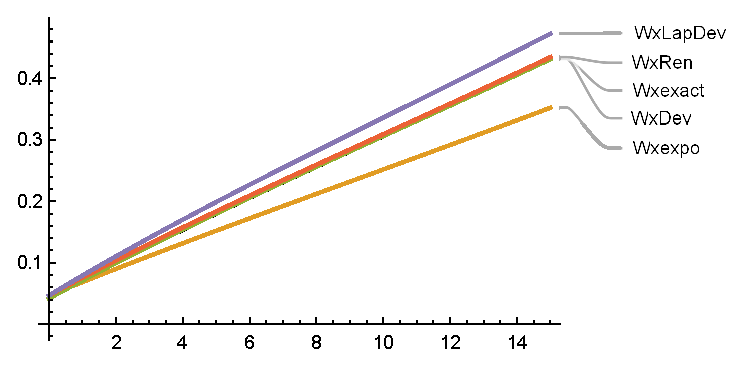
\includegraphics[width=\textwidth]{AzcueMW}
        \caption{$W_q(x)$  (in black)}
        \label{fig:AzcueMW}
    \end{subfigure}
    ~
    \\
    \begin{subfigure}[b]{0.8\textwidth}
        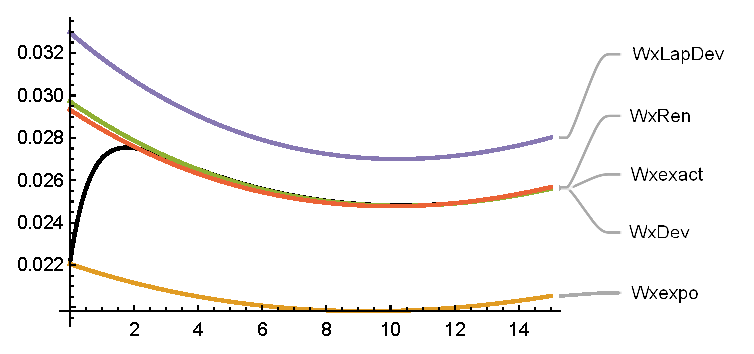
\includegraphics[width=\textwidth]{AzcueMW1}
        \caption{$W'_q(x)$}
        \label{fig:AzcueMW1}
    \end{subfigure}
    ~
    \\
    \begin{subfigure}[b]{0.8\textwidth}
        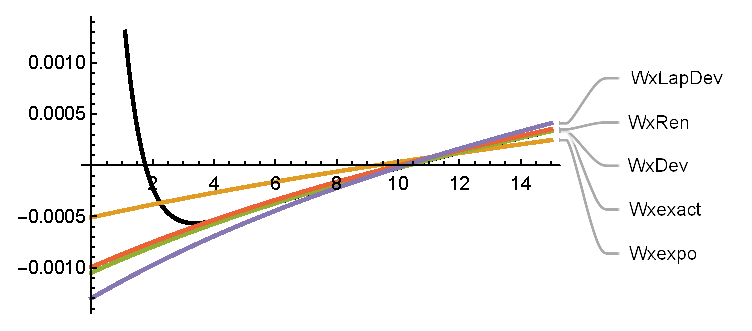
\includegraphics[width=\textwidth]{AzcueMW2}
        \caption{$W''_q(x)$}
        \label{fig:AzcueMW2}
    \end{subfigure}
    \caption{Plots of $W_q(x)$, $W'_q(x)$, and $W''_q(x)$ of the exact solution and the approximations for $f(x) = 10 \le(x e^{-x}\ri)$, $\th = \frac{7}{100}$, $q=\fr{1}{10}$.}\label{fig:AzcueM}
\end{figure}


\begin{table}[!h]
\begin{tabular}{|l|l|l|l|l|}
\hline
       & \begin{tabular}[c]{@{}l@{}}Dominant   exponent \\ $\Phi_q$\end{tabular} & \begin{tabular}[c]{@{}l@{}}Percent   relative error\\ ($\Phi_q$)\end{tabular} & \begin{tabular}[c]{@{}l@{}}Optimal barrier\\ $b_{DeF}$\end{tabular} & \begin{tabular}[c]{@{}l@{}}Percent   relative error\\ ($b_{DeF}$)\end{tabular} \\ \hline
Exact  & 0.142175                   & 0                                 & 2.61925              & 0                             \\ \hline
Expo   & 0.139202                   & 2.09118                           & 2.79162              & 6.58074                       \\ \hline
Dev    & 0.142174                   & 0.00104491                        & 2.60329              & 0.609153                      \\ \hline
Renyi  & 0.142238                   & 0.0439717                         & 2.59638              & 0.873044                      \\ \hline
LapDev & 0.143232                   & 0.743272                          & 2.48327              & 5.19155                       \\ \hline
\end{tabular}
\caption{Exact and approximate values of $\Phi_q$ and $b_{DeF}$ for $f(x) = 10 \le(x e^{-x}\ri)$, $\th = \frac{7}{100}$, $q=\fr{1}{10}$. The DeVylder approximation displayed the least percent relative error among the four approximations considered.}
\label{table:AzcueM}
\end{table}